\documentclass[11.5pt]{article}
        \usepackage{graphicx,type1cm,eso-pic,color}
        \usepackage{hyperref}
        \usepackage[left=3.0cm,right=3.0cm,top=2cm,bottom=2cm,headheight=13.6pt]{geometry}
       %\usepackage{subfigure}

\makeatother
\begin{document}

\rightline{December 2 2016}
\rightline{Version V1.0}
\vskip 0.5cm
\begin{center}

\begin{figure}[htbp]
\begin{center}
\vspace{0cm}
\includegraphics[scale=0.3]{pics/ft-drawing.eps}
\end{center}
\end{figure}

\vskip 1.5cm

{\huge\bf\bf CLAS12}
\vskip 0.5cm

{\huge\bf\bf Forward Tagger Calorimeter (FT-Cal)}
\vskip 0.5cm


{\huge\bf Manual of operation}
\vskip 0.8cm
{\large\bf The CLAS12 Collaboration}
\vskip 0.5cm
\end{center}

\vskip 1.5 cm
\abstract{
This operation manual would it be the short-cut to access the FT-Cal operations for the users.
It contains all the information to operate the detector during data taking or maintenance period. An overview on the HV, LV and cooling systems is reported.
}
\vskip 0.5cm

\newpage

\title{Short Manual for CLAS12 FT-Cal v2.0} 

\maketitle{}

\tableofcontents

\newpage


\section{Requirements}
All users MUST have:\\
\begin{itemize}
\item   a valid JLab account 
\item   use the \textbf{clasrun} user for all instructions in this document
\end{itemize}
This manual is for users only. If you are an expert, refers to the main manual~\cite{manual} or in the tdr for more information \cite{ftacl-tdr}.

\section{The EPICS main control panel}  
All FT detectors are controlled via EPICS from a single panel shown in Fig.~\ref{fig:EPICSmain}. The FT-Cal detector is one of the FT sub-systems and all operations are accessible from the same panel.\\
To execute the panel, digit the following command from a terminal of the \texttt{clonpc\#\#} workstations in the Hall-B counting house:
\begin{center}
\texttt{clas12\_epics}
\end{center}
and select the FT-Cal panel from the FT tab in Fig.~\ref{fig:EPICSmain} to access to all services:
\begin{itemize}
\item \textbf{\textit{FTC Overview:}} High voltage and low voltage controls, monitor of the temperature sensors and chiller temperature monitor and control
\item \textbf{\textit{FTC Flasher Expert:}} Management of the LED FT-Cal system for expert use only
\item \textbf{\textit{FTC Flasher Novice:}} Management of the LED FT-Cal system for users and normal operation
\item \textbf{\textit{FTC Gas}} Nitrogen control system
\end{itemize}    
%\%\%\%\%\%\%\%\%\%\%\%\%\%\%\%\%\%\%\%\%\%\%\%\%\%\%\%\
\begin{figure}[ht!]
\center
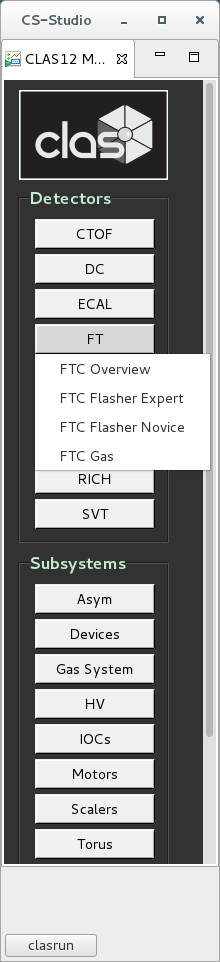
\includegraphics[width=0.13\textwidth]{pics/clascss_main_menu_FT_selection.png}
\caption{ \label{fig:EPICSmain} View of the Hall-B EPICS main window. Menu shown gives access to all control panels.}
\end{figure}
%\%\%\%\%\%\%\%\%\%\%\%\%\%\%\%\%\%\%\%\%\%\%\%\%\%\%\%\

\subsection{The FTc Overview panel}\label{sec:ft-epics}
The panel shows the FT-Cal overview and the user can immediately appreciate the status of the detector. The grey square buttons in the top right of each section of the main FT-Cal screen provide
access to more detailed or expert screens for the corresponding subsystem.
%\%\%\%\%\%\%\%\%\%\%\%\%\%\%\%\%\%\%\%\%\%\%\%\%\%\%\%\
\begin{figure}[ht]\centering
    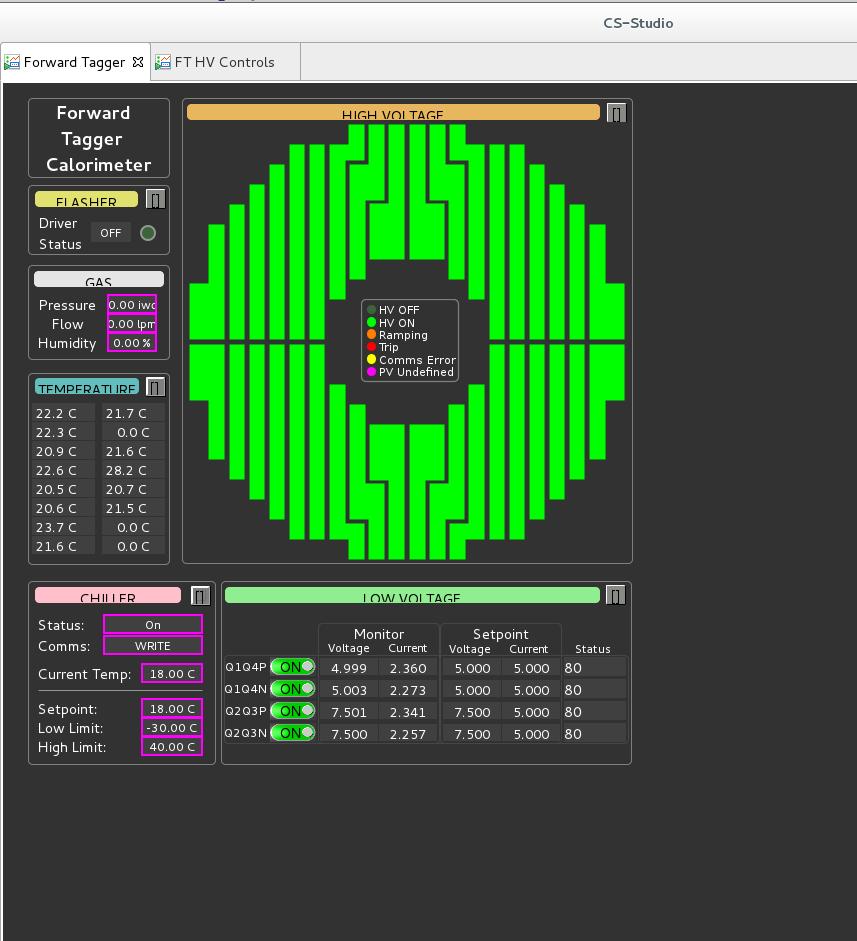
\includegraphics[width=8cm]{pics/All_Working_HVs.png}
    \caption{The primary EPICS screen needed for shift workers to monitor FT-Cal.\label{fig:ecal_all}}
\end{figure}

\subsubsection{Temperature}\label{sec:ft-t}
\textbf{The FT-Cal temperature should remain stable within $\pm 0.1^{\circ}$ C} in order to avoid gain variation in the system.\\
\textbf{\textit{Variations of one Celsius degree ($^{\circ}$C) or more during a shift should be reported to FT-Cal expert on call and noted in the log book.}}
\begin{itemize}
\item \textit{\textbf{Temperature Sensors:}} There are 16 temperature sensors in the FT-Cal enclosure to be monitored. Clicking on the grey square button in the top right of the temperature section the expert panel in  Fig.~\ref{fig:temp} pops up. The strip charts shown in Fig.~\ref{fig:striptemp} are accessible from the two buttons in the temperature section of Figure ~\ref{fig:ecal_all}.
\end{itemize}
%\%\%\%\%\%\%\%\%\%\%\%\%\%\%\%\%\%\%\%\%\%\%\%\%\%\%\%\
\begin{figure}[ht]
\center
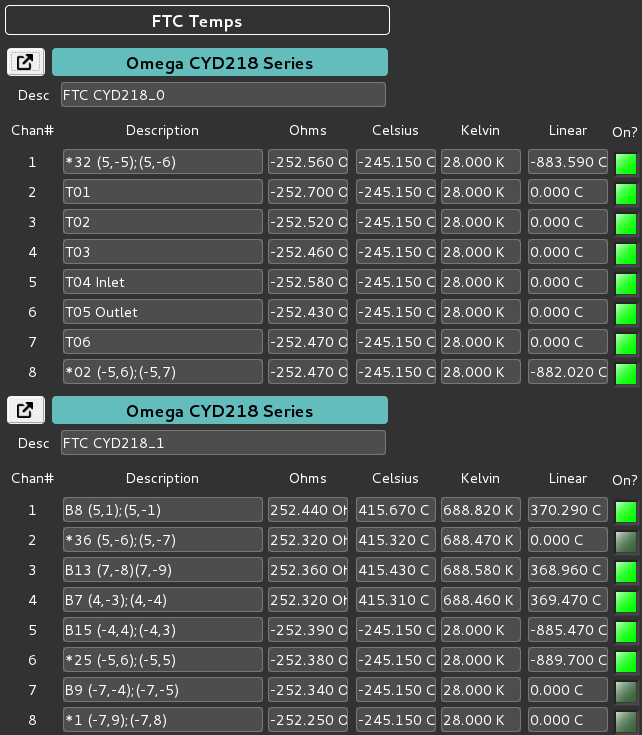
\includegraphics[width=0.4\textwidth]{pics/PT100_3.png}
\caption{ \label{fig:temp} View of the EPICS temperature monitoring window.}
\end{figure}

\begin{figure}[ht]
\center
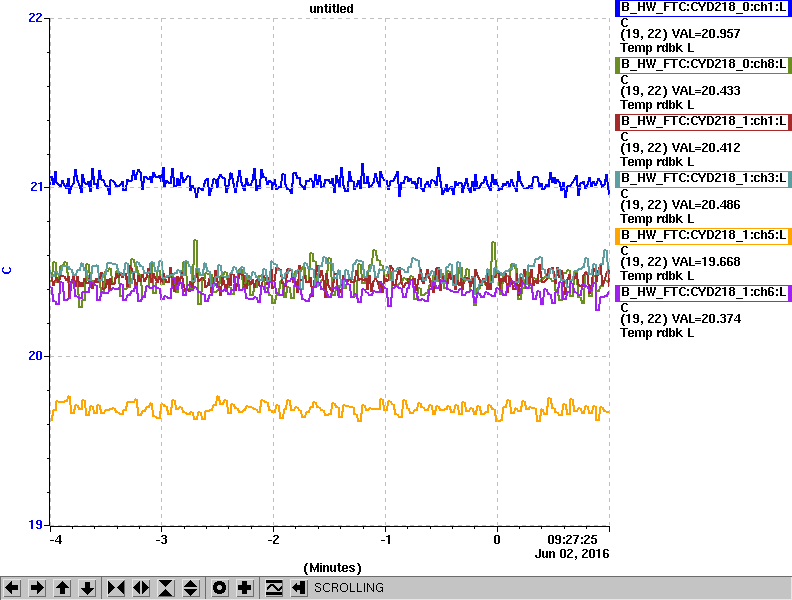
\includegraphics[width=0.45\textwidth]{pics/Strip_Chart_T_Crystal.png}
\caption{ \label{fig:striptemp} Example view of what the implemented EPICS strip charts will look like}
\end{figure}
%\%\%\%\%\%\%\%\%\%\%\%\%\%\%\%\%\%\%\%\%\%\%\%\%\%\%\%\

\subsubsection{Chiller}\label{sec:ft-chiller}
\textbf{The chiller MUST be ONduring data taking.}\\ 
It allows to keep the calorimeter at the temperature of -3 C. The chiller can be monitored through the EPICS control (Figure~\ref{ChillerCam}). 
\textit{\textbf{Shift takers should not attempt to change the chiller settings. Call FT-Cal expert in case of problem.}}
\begin{figure}[ht]
\center
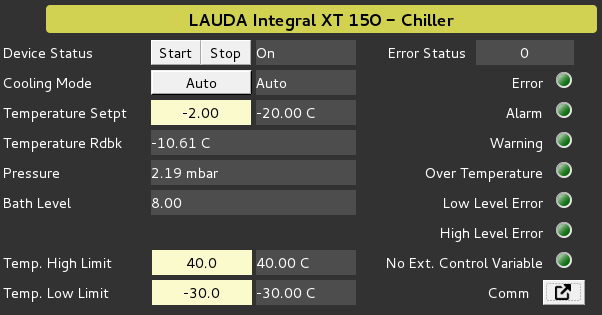
\includegraphics[width=0.5\textwidth]{pics/Chiller_Slwcntrl.png}
\caption{ \label{ChillerCam} View of the chiller slow control window.}
\end{figure}
%\%\%\%\%\%\%\%\%\%\%\%\%\%\%\%\%\%\%\%\%\%\%\%\%\%\%\%\

\subsubsection{Low Voltage}\label{sec:ft-lv}
\textbf{The low voltage power supply must be ON before HV is turned on.\\} 
\textbf{\textit{Changing HV settings requires contact with an FT-Cal-expert.\\}}
\textbf{The currents driven by the four channels should be similar. Normal current is between 2.2 and 2.4 A for all channels.\\}
\textbf{\textit{Call the FT-Cal expert if this appears not to be ON or shows an abnormal current for any of the channels.}} 
%\%\%\%\%\%\%\%\%\%\%\%\%\%\%\%\%\%\%\%\%\%\%\%\%\%\%\%\
\begin{figure}[ht]
\center
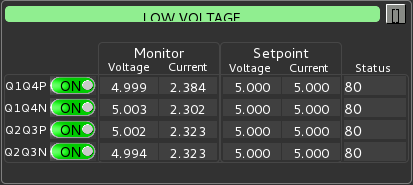
\includegraphics[width=0.3\textwidth,height=3.5cm]{pics/LV.png}
\caption{ LV controls for the FTCal. }
\end{figure}
%\%\%\%\%\%\%\%\%\%\%\%\%\%\%\%\%\%\%\%\%\%\%\%\%\%\%\%\
\newpage
\section{High Voltage}\label{sec:ft-hv}
\subsection{Turning ON/OFF High Voltages}
\textbf{HV should be turned on always after LV. \\
During data-taking also the chiller have to be ON.\\} 
Open the HV expert panel clicking on the grey top button of the HV panel in the FT-Cal
EPICS window (Figure ~\ref{fig:ecal_all}).\\
In the expert panel it is possible to choose :
\begin{itemize}
\item rump up and down the entire calorimeter
\item rump up and down single channels opening a more detailed panel in Fig.~\ref{fig:HVControl}
\item monitor the HV trend using the strip chart in Fig.~\ref{fig:hvcurrentstrips}.
\end{itemize}
\textit{\textbf{ Jumps or drifts in current of more than 1 A should be noted in the logbook.}}\\
%\%\%\%\%\%\%\%\%\%\%\%\%\%\%\%\%\%\%\%\%\%\%\%\%\%\%\%\
\begin{figure}[ht]
\center
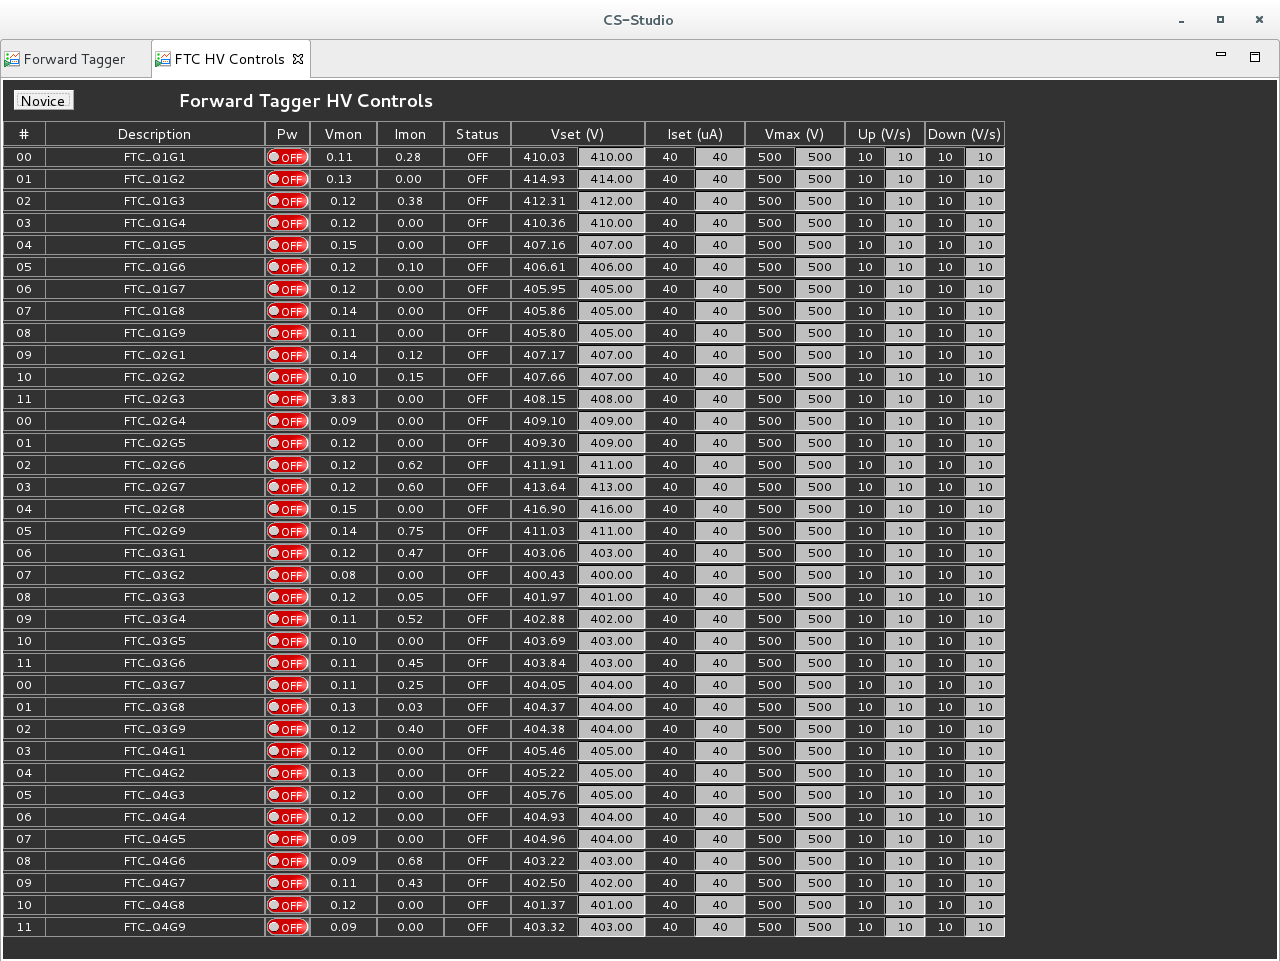
\includegraphics[width=0.72\textwidth]{pics/FTC_HV_controls_expert.png}
\caption{ \label{fig:HVControl} View of the EPICS FT-Cal HV control window for individual channels.}
\end{figure}
%\%\%\%\%\%\%\%\%\%\%\%\%\%\%\%\%\%\%\%\%\%\%\%\%\%\%\%\

%\%\%\%\%\%\%\%\%\%\%\%\%\%\%\%\%\%\%\%\%\%\%\%\%\%\%\%\
  \begin{figure}[htbp]\centering
       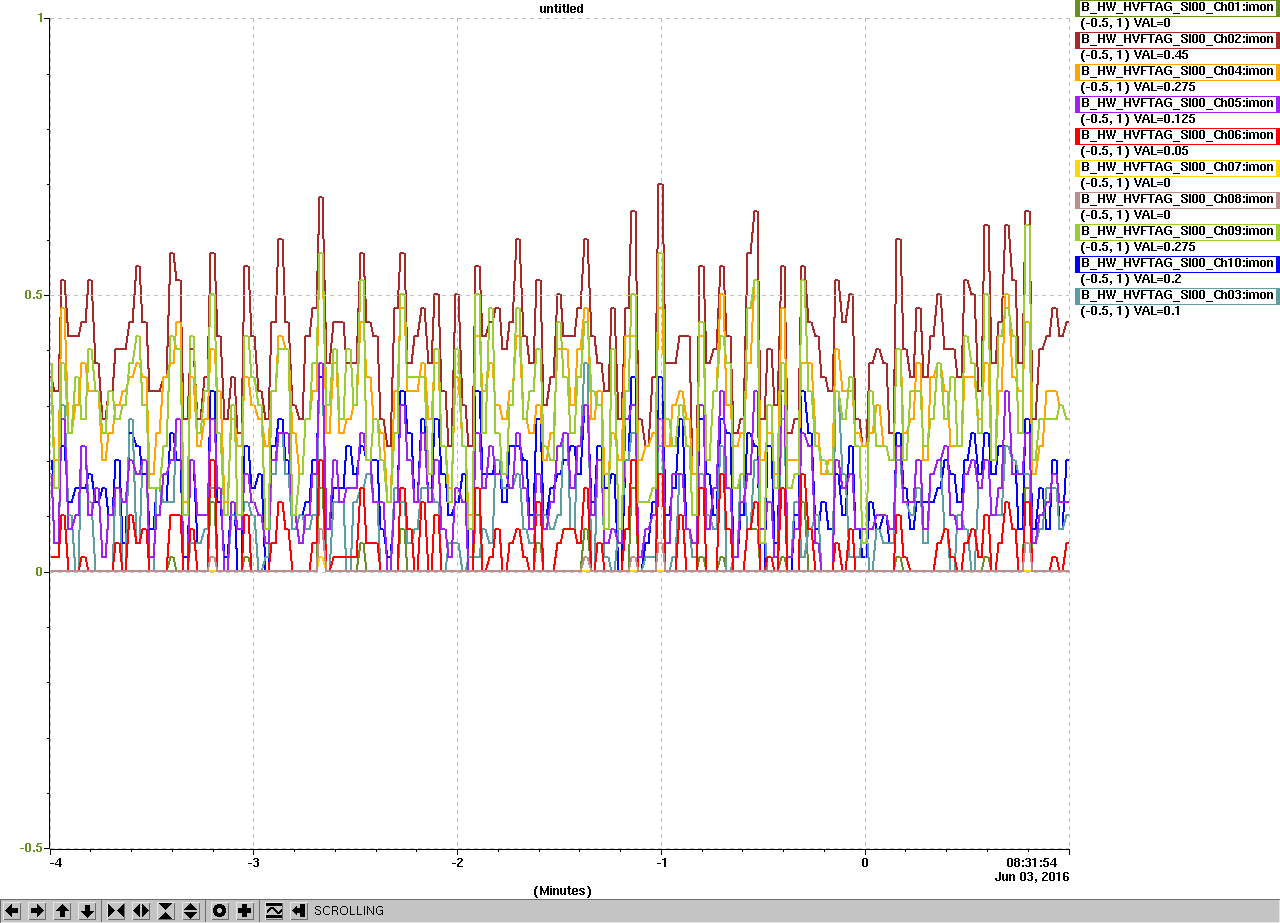
\includegraphics[width=8.4cm]{pics/HV_I_Strip_Chart.png}
       \caption{Example HV Current strip chart.\label{fig:hvcurrentstrips}}
  \end{figure}
%\%\%\%\%\%\%\%\%\%\%\%\%\%\%\%\%\%\%\%\%\%\%\%\%\%\%\%\
In case of HV trip the correspondent HV group in the main panel turns to red. HV trips will also be announced by the alarm handler.  During normal operations with HV ON, there should be no red groups in Fig.~\ref{fig:ecal_all} and no ECAL HV alarms.\\  
In case of an HV trip, or a red region in Figure \ref{fig:ecal_all}:
\begin{itemize}
    \item try to re-enable the tripped HV group by turning it back on as described before.
    \item record the trip in the log book with precise indication of the group and run
        number concerned.
\end{itemize}
\textcolor{red}{\textbf{Contact the FT-CAL expert on-call in case of uncertainty.}}\\
 {\em Note, the HV can take up to 1 minute to turn back on so you should end the current run and begin a new one when the high voltage is back on.} \\ 
 \textbf{If you cannot get a HV group to work contact the FT-Cal expert on call.}\\
 {\bf If you encounter more than two HV trips during your shift for the same group, you should notify the FT-Cal Expert.}

 \section{Scalers}      
Rates seen by the FT-Cal are available in the ROOT-based GUI shown in Fig.~\ref{Scalers}.\\
\textbf{Rates should remain constant within $^\sim10\%$ during stable beam operation.}\\
\textit{\textbf{A strong increase is the indication of bad beam conditions or the presence of a new source of noise in the FT-Cal system.  If the latter case, please contact FT-Cal expert on call.}}\\
The Scaler Gui is stored on the jlab12daq1 machine.   
%\%\%\%\%\%\%\%\%\%\%\%\%\%\%\%\%\%\%\%\%\%\%\%\%\%\%\%\      
\begin{figure}[htbp]
\center
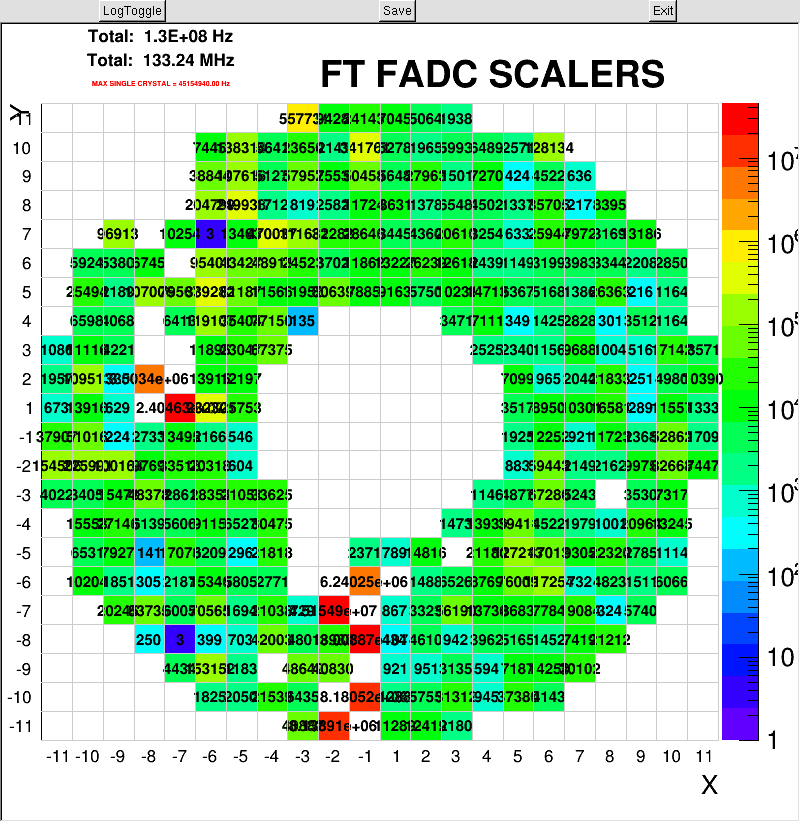
\includegraphics[width=0.5\textwidth]{pics/Scalers.png}
\caption{ \label{Scalers} View of the EPICS FADC scalers window (to be updated based on beam-commissioning rates.}
\end{figure}
%\%\%\%\%\%\%\%\%\%\%\%\%\%\%\%\%\%\%\%\%\%\%\%\%\%\%\%\

\section{Strip Charts}
The most import quantities to monitor with strip charts are temperature and HV current.  
The StripTool from MyaViewer, shown in Figure~\ref{fig:striptemp}, runs by executing the following scripts in a terminal (To Be Implemented):
      \begin{itemize}
          \item \texttt{mya\_ftcal\_all.sh}
          \item \texttt{mya\_ftcal\_temp.sh}
          \item \texttt{mya\_ftcal\_curr.sh}
          \item \texttt{mya\_ftcal\_voltage.sh}
      \end{itemize}

\newpage
\section{How to switch ON/OFF the FT-Cal}
The FT-Cal to operate requires to have the LV, HV and the chiller on. \\

\subsubsection{Switching the FT-Cal ON}
\begin{itemize}
\item{From  the CLAS12 EPICS control bring the primary FT-Cal EPICS screen ON (see Sec.\ref{sec:ft-epics} )}
\item{Check temperatures (see Sec.\ref{sec:ft-t}) and the status of the chiller (see Sec.\ref{sec:ft-chiller}), if OFF, do not proceed and  call the FT-Cal expert.}
\item{Switch the LV ON (see Sec.\ref{sec:ft-lv})}
\item{Switch the HV ON (see Sec.\ref{sec:ft-hv}) {\it HV has to  be switched ON AFTER LV!}}
\end{itemize}

\subsubsection{Switching the FT-Cal OFF}
\begin{itemize}
\item{From  the CLAS12 EPICS control   bring the primary FT-Cal EPICS screen ON (see Sec.\ref{sec:ft-epics} )}
\item{Switch the HV OFF (see Sec.\ref{sec:ft-hv}) {\it HV has to  be switched OFF BEFORE LV!}}
\item{Switch the LV OFF (see Sec.\ref{sec:ft-lv}).}
\item{Leave the chiller ON (see Sec.\ref{sec:ft-chiller})}
\end{itemize}

\section{The FT-Cal data monitor}
The application used to monitor on-line and off-line data provides plots to assess detector performance.\\  
To start the monitoring app, in a terminal run:
\begin{center}
\texttt{clas12-module}
\end{center}
\begin{itemize}
\item choose from the menu the monitoring application you are interested in
\item click the ``Et'' button to connect to the ET ring
\item click the ``$>>$'' to start the event processing
\item at the start of every run, clear the histograms via the ``Clear Histograms''
\end{itemize}
After a few minutes of beam, the tabs should be cycled through and their plots compared to the reference.  Once sufficient statistics are accumulated, snapshot of the relevant panel should be taken and uploaded to the logbook.

\section{The LED run}
The LED system is operated through an EPICS GUI accessible from the main CLAS12 EPICS menu, through FT, then FTC-Flasher Novice (see Figure \ref{FlasherMEDM}).\\
\textbf{\textit{Shift takers are requested to operate the system in ``Sequence mode'' only.}} \\
The sequence:
\begin{itemize}
\item click on ``Initialize Flasher''
\item verify the TOP frequency is 8000 Hz (if necessary adjust it trough the proper drop-down menu)
\item click on ``Start''
\end{itemize}
During such a run the DSC scaler screen and the monitoring app allows to check the proper functioning of the channels.
%\%\%\%\%\%\%\%\%\%\%\%\%\%\%\%\%\%\%\%\%\%\%\%\%\%\%\%\
\begin{figure}[htbp]
\center
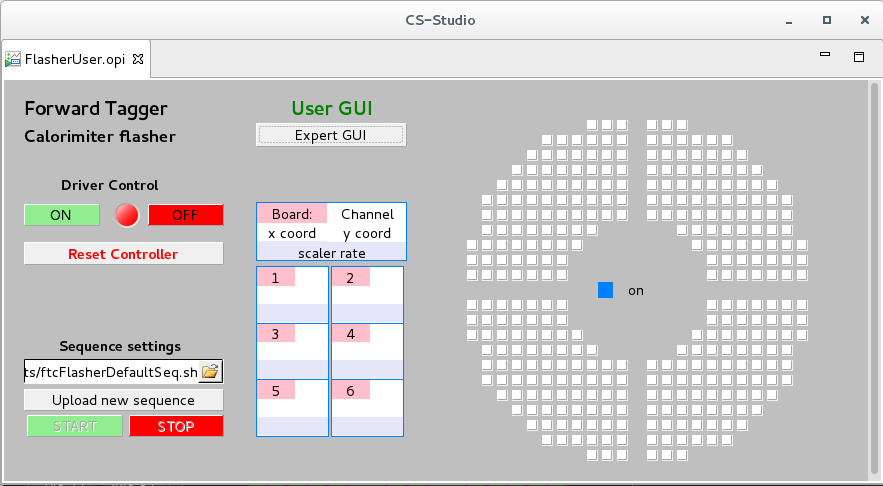
\includegraphics[width=0.7\textwidth]{pics/FTC_flasher.png}
\caption{ \label{FlasherMEDM} The FT-CAL Led monitoring system EPICS GUI.}
\end{figure}

\subsection{Taking a LED sequence run}
This involves setting the DAQ, starting the LED sequence run, and configure the  monitoring app to monitor the data. At the end of the run, the user can upload the relevant information to the CLAS12 conditions database, as well as post a log-entry to the HallB electronic logbook.

\subsubsection{Setup}
It is critical they are followed in the \textbf{exact} order as they are here reporter.
\begin{enumerate}
\item{\textbf{Start the DAQ system: }
\begin{itemize}
\item Identify the machine where the DAQ RunControl is running. 
\begin{itemize}
\item If the DAQ system is not available, it has to be initialized from scratch. \textit{Refer to the CLAS12 DAQ manual, or contact the DAQ expert.}
\end{itemize}
\item Depending on the DAQ state, different buttons may be visible in the ``Transition'' area. If the ``Configure'' button is not visible, click on ``Reset'', then on ``OK''.
\item Click on ``Configure'' to properly set up the run.
A ``Run Type Configuration'' dialog will show up.

There are two active FT  configurations available: 
\begin{itemize}
\item{FT: this is the standard configuration; all CODA modules are up, FT data are collected and written on disk.}
\item{FT\_NOER: CODA ER module is off, data are collected for on-line analysis but they are not saved on disk.}
\end{itemize}

\item{Click on ``Download'' button. A file-chooser menu will show up.

Select: clasdev.trg. 

Click on ``OK'' to close the file-choose menu.
}
\item{Click on ``Prestart''.  Wait until the ``GO'' button appears, but {\bf do not click on it yet.}

 }
\end{itemize}
}
\item{\textbf{Start the monitoring app: }Use the command clas12-module on a terminal to start the monitoring app and select the FTCalViewerModule.

\textcolor{red}{\bf Do this after the run-control shows the ``GO'' button.}

When the monitoring gui window shows up, click on the {\it Et} button to connect to the ET ring and on the ``$>>$'' button to start the event processing. }
\item{\textbf{Initialize the LED monitoring sequence:} In the EPICS gui, click on ``Initialise Flasher'', ``Start Flasher'', then on ``!Stop All Seq'' (to ensure there are no previous sequences running). 
}
\end{enumerate}
      
\subsubsection{Run start, data taking, and run stop}
To start data taking follow these instructions, in the exact order they are reported here.
\begin{enumerate}
\item In the RunControl GUI, click on the ``GO'' button. Wait 10~s, until the message ``transition go succeeded'' is displayed in the log window and the ``END'' button displays. 
\item In the EPICS LED GUI, click on ``Start''.
\item To stop the run when the sequence is ended click on "END".
\end{enumerate}

While the LED sequence is running, you can look at the monitoring application to check data being recorded. \\
\textit{The event display will show 6 crystals at time with a signal and a full sequence will take $\simeq$ 50 minutes to complete.}\\
\textit{Use the EPICS gui to periodically check the sequence status, looking at the Sequence Control section (RED is OFF, GREEN is ON). }\\
{\bf  The DAQ system is not set up to end the run when the LED sequence is completed.} When the sequence is complete:
\begin{itemize}
\item The LED system automatically turns off. As a direct consequence of this, no further triggers are sent to the DAQ system
\item The data-taking run is \textbf{not} ended. This means the DAQ will stay in RUN mode, but no events will be recorded, since there are no triggers.
\end{itemize}

The user can confirm the sequence has actually ended by looking at the FT-Cal Event display: no crystals have signal when the sequence is off.

When the sequence is OFF, first turn OFF the controller (LED ON/OFF, click on OFF), 
then use the DAQ run control to END the run, by clicking on the ``End'' button.

\subsubsection{Analysis of the LED run}
When the run ends, loop through the different tabs of the monitoring application to check the histograms were correctly filled. \\
\textit{\textbf{Check in particular that no calorimeter channel in this map is shown as grey that would indicate the channel is dead or the sequence was not complete. In that case  contact the FT-Cal expert on call.}}

Close and restart the monitoring application and analyze the recorded EVIO file by selecting it via the ``File'' button. 

Once the analysis is completed, loop again through the different tabs to verify histograms an calorimeter maps. Check the values reported on the ``Charge'' tab:  the average channel response should be in the range $\simeq 20 \div 30$.  Make an entry in the e-logbook , reporting the run number and including a snapshot of the ``Charge'' tab and the LED calibration result file. The path to the latter will be indicated on the terminal from which the monitoring application was started.

\section{Noise Run}
A quick check of the calorimeter channels functionality can be obtained with a quick LED run. We simply use the LED sync trigger to have data recorded without performing a full LED sequence and check the noise levels recorded for each channels.\\ 
\textbf{A channel is operating normally if the noise RMS is within 0.75 and 1.1 mV. Noise below this range may indicate the channel is dead. If this is the case reports on the logbook.}

In order to perform this check, set the sequence: 

\begin{enumerate}
\item{\textbf{Start the DAQ system: }}
\begin{itemize}
\item Identify the machine where the DAQ RunControl is running. If you can't find it anywhere, it is possible the DAQ system has to be initialized from scratch. To do so, refer to the CLAS12 DAQ manual, or contact the DAQ expert.
\item Depending on the DAQ state, different buttons may be visible in the ``Transition'' area. If the ``Configure'' button is not visible, click on ``Reset'', then on ``OK''.
\item Click on ``Configure'' to properly set up the run. A ``Run Type Configuration'' dialog will show up. Use the scroll-down menu to select as RunType: FT. This configuration will also save any data on tape. Use instead: FT\_NOER to not save data on tape.

\textit{Default is to save data to the tape}
\item{Click on ``Download'' button. A file-chooser menu will show up.

Select: clasdev.trg. 

Click on ``OK'' to close the file-choose menu.
}
\item{Click on ``Prestart''.  Wait until the ``GO'' button appears.}
\item{In the RunControl GUI, click on the ``GO'' button. Wait 10~s, until the message ``transition go succeded'' is displayed in the log window and the ``END'' button displays.}
\end{itemize}

\item{\textbf{Initialize the LED monitoring sequence:}In the EPICS gui, click on ``Initialise Flasher'', then on ``!Stop All Seq'' (to ensure there are no previous sequences running) and finally on ``Start''. }
\item{\textbf{Start the monitoring app: }}
\begin{itemize}
\item{Use the command outlined in the previous section to start the monitoring app. When the monitoring gui window shows up, click on the ``Et'' button to connect to the ET ring and on the ``$>>$ button to start the event processing. }
\item{Accumulate events for 2 minutes.}
\item{Go to the ``Noise'' ~\ref{fig:NOISE-MAP}
    tab and check the detector view map on the left panel: noise levels are within range if they show in green.}
\item{Compare the color map with previous ones to verify the presence of new ``dead'' (blue) or ``noisy'' channels (orange). Take a snapshot of the panel and make an e-logbook entry with the appropriate comments.}

\begin{figure}[ht]\centering
    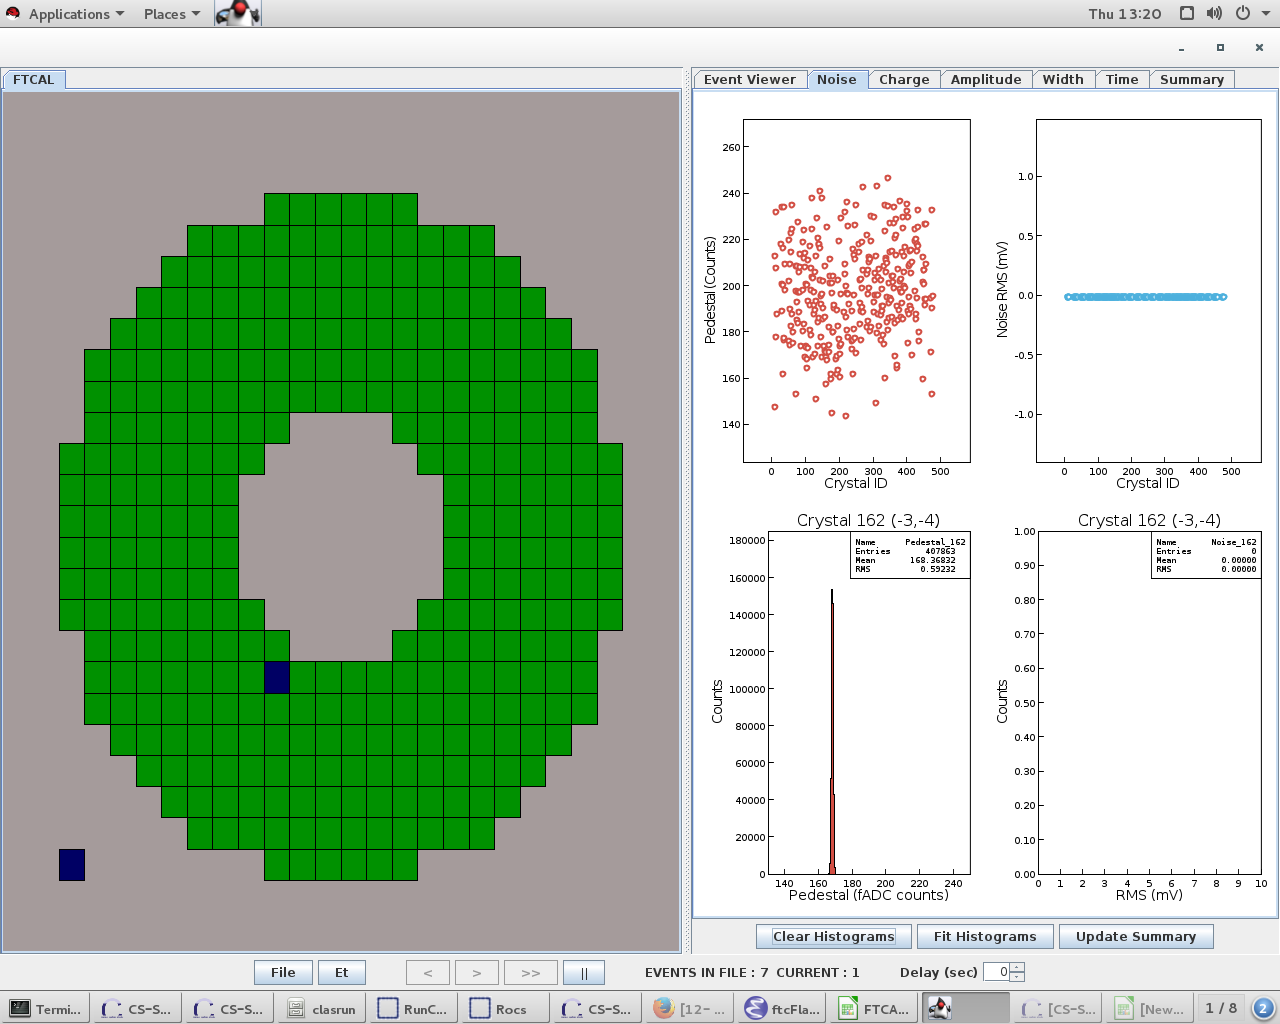
\includegraphics[width=9cm, height=6cm]{pics/NOISE_MAP.png}
    \caption{Example Noise map within the LED monitoring Gui. The color of the heat map is determined by the RMS of the mean of the noise of a given channel.\label{fig:NOISE-MAP}}
\end{figure}
  
\item{\textit{\textbf{If new problematic channels are found, contact the FT-Cal expert on call.}}}
\end{itemize}
\item{\textbf{Stop the DAQ:} click on ``End Run''. }
\item{\textbf{Stop the LED controller:} end the sequence by clicking on ``Stop'' and turn off the drivers by clicking on ``OFF''. }
\end{enumerate}


\section{Taking a Cosmic Calibration Run}
\begin{enumerate}
\item{\textbf{Start the DAQ system: }}
\begin{itemize}
\item Identify the machine where the DAQ RunControl is running. If you can't find it anywhere, it is possible the DAQ system has to be initialized from scratch. To do so, refer to the CLAS12 DAQ manual, or contact the DAQ expert.
\item Depending on the DAQ state, different buttons may be visible in the ``Transition'' area. If the ``Configure'' button is not visible, click on ``Reset'', then on ``OK''.
\item Click on ``Configure'' to properly set up the run. A ``Run Type Configuration'' dialog will show up. Use the scroll-down menu to select as RunType: FT. This configuration will also save any data on tape. Use instead: FT\_NOER to not save data on tape. ~\ref{fig:SELFTRIG1}

%\%\%\%\%\%\%\%\%\%\%\%\%\%\%\%\%\%\%\%\%\%\%\%\%\%\%\%\
\begin{figure}[htbp]\centering
     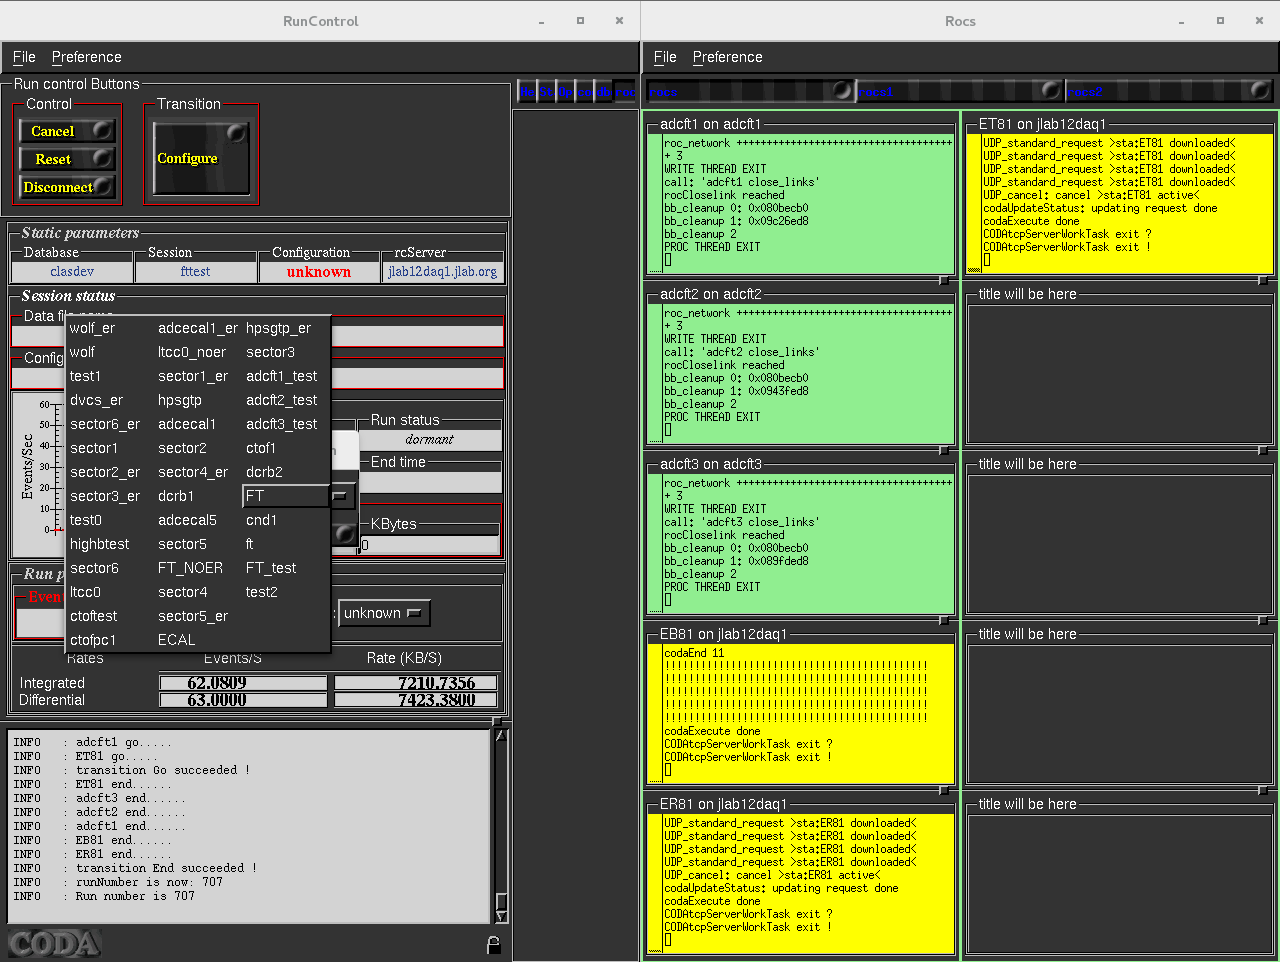
\includegraphics[scale=0.33]{pics/SELF_TRIGGER_0.png}
     \caption{Depending on whether the user would like to record or only view live data, there are two configuration options to choose from. The FT option records data, and the FT\textunderscore NOER option only shows live events. \label{fig:SELFTRIG1}}
\end{figure} 
%\%\%\%\%\%\%\%\%\%\%\%\%\%\%\%\%\%\%\%\%\%\%\%\%\%\%\%\

\textit{Default is to save data to the tape}
\item{Click on ``Download'' button. A file-chooser menu will show up.
  On the Left pane of the popup window select .../parms/trigger/FT
  Once within the aforementioned directory Select ft\_selftrigger.trg in the Right pane

  Click on ``OK'' to close the file-choose menu. \ref{fig:SELFTRIG2}}

%\%\%\%\%\%\%\%\%\%\%\%\%\%\%\%\%\%\%\%\%\%\%\%\%\%\%\%\
\begin{figure}[htbp]\centering
  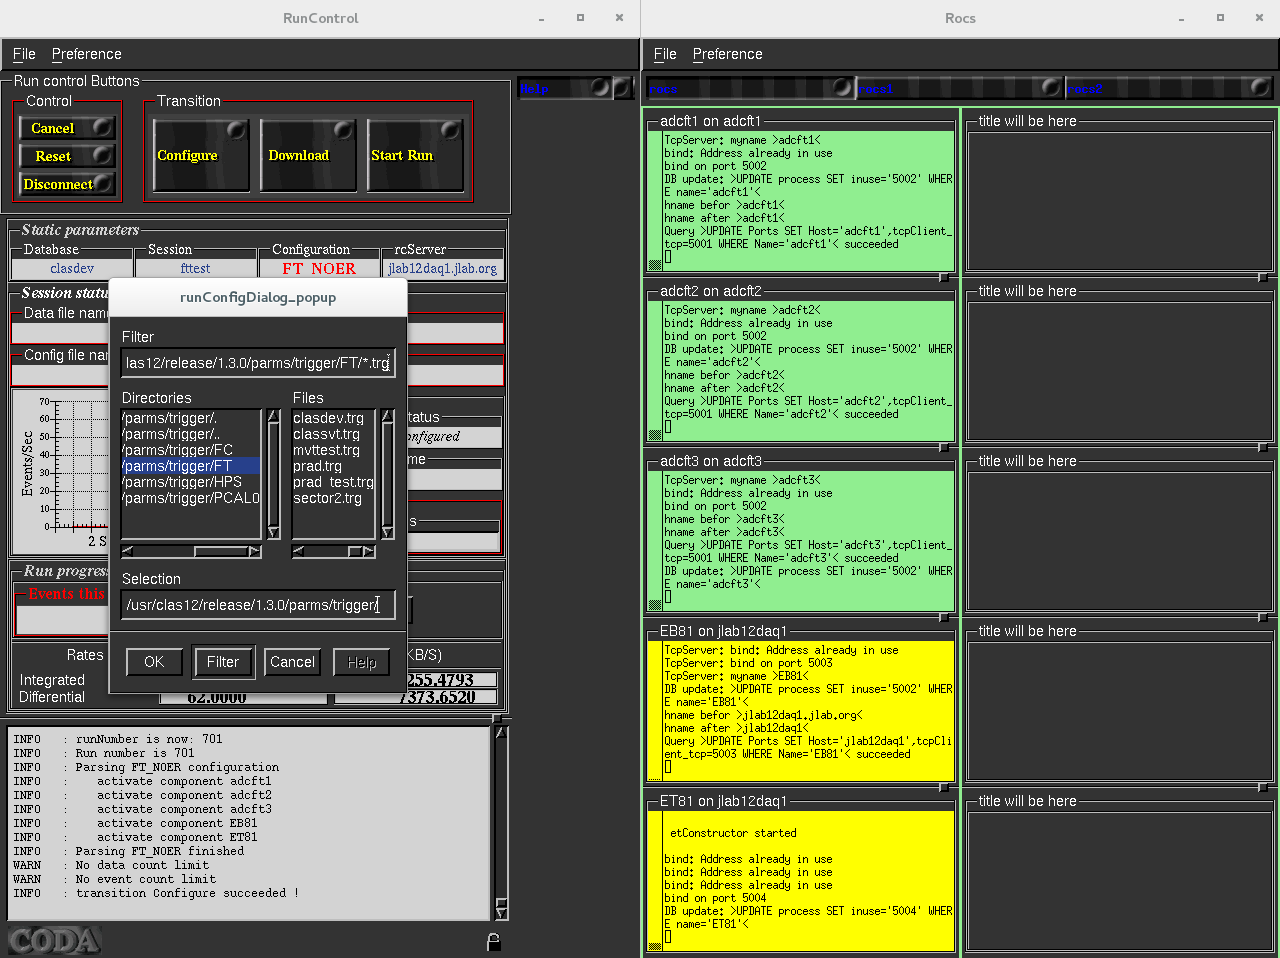
\includegraphics[scale=0.3]{pics/SELF_TRIGGER_1.png}
  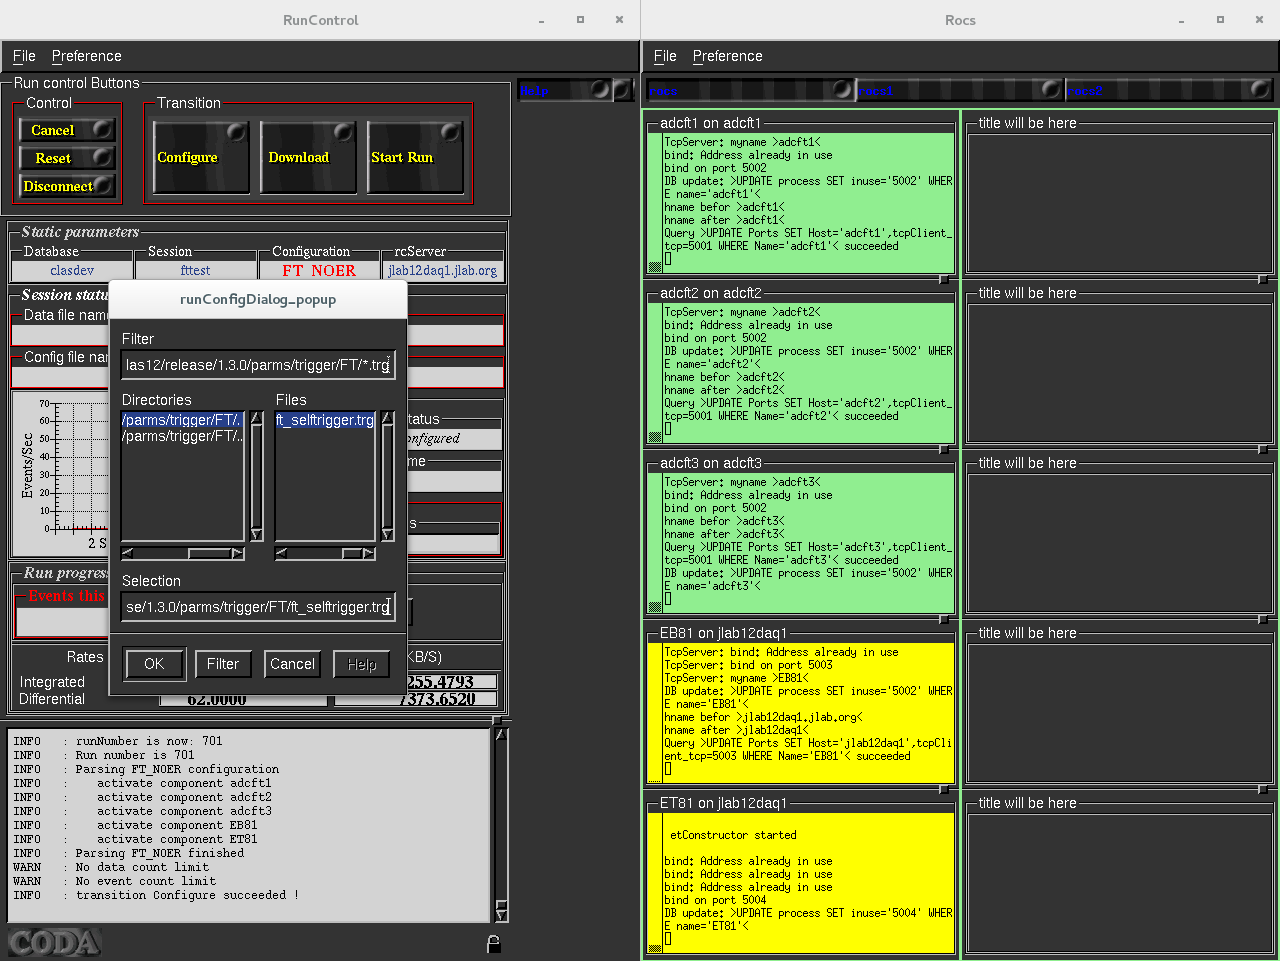
\includegraphics[scale=0.3]{pics/SELF_TRIGGER_2.png}
     \caption{Once the configuration has been chosen, the user will then download the corresponding trigger file. In the case of the Forward Tager, this file is accessed by clicking the download button and navigating to .../parms/trigger/FT/ in the left window of the popup, and selecting the file called ft\textunderscore selftrigger.trg in the right window.
       \label{fig:SELFTRIG2}}
\end{figure} 
%\%\%\%\%\%\%\%\%\%\%\%\%\%\%\%\%\%\%\%\%\%\%\%\%\%\%\%\

\item{Click on ``Prestart''.  Wait until the ``GO'' button appears.}
\item{In the RunControl GUI, click on the ``GO'' button. Wait 10~s, until the message ``transition go succeded'' is displayed in the log window and the ``END'' button displays.}
\end{itemize}
\item{\textbf{Start the monitoring app: }}
\begin{itemize}
\item{Use the command outlined in the previous section to start the monitoring app. When the monitoring gui window shows up, click on the ``Et'' button to connect to the ET ring and on the ``$>>$ button to start the event processing. }
\item{Once connected to the ET ring the user will see live events on the Left pane of the monitoring app\ref{fig:CROSSING}, as well as the waveform and tabs to provide further analysis on the Right.}
\end{itemize}

\begin{figure}[htbp]\centering
  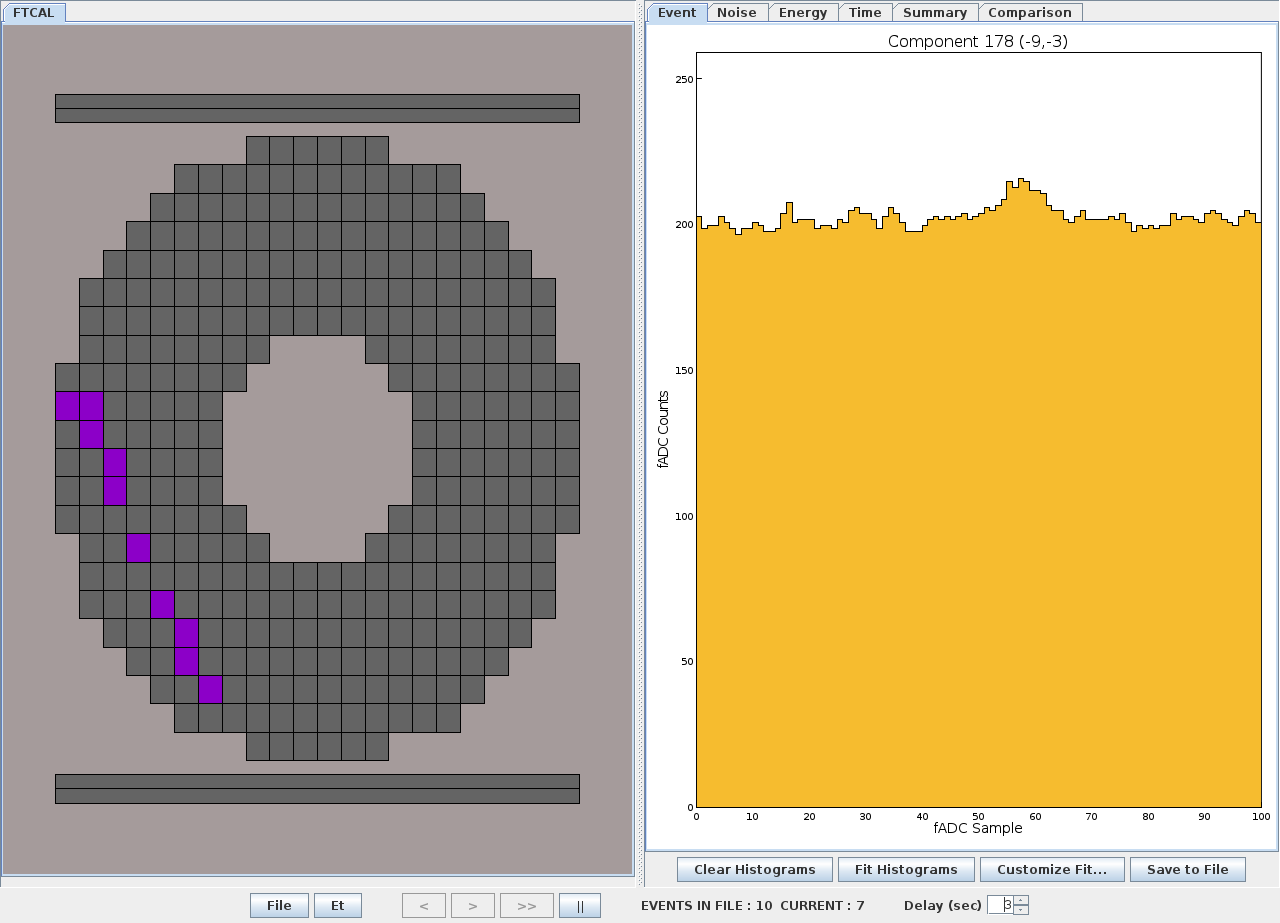
\includegraphics[width=12cm, height=7cm]{pics/Success_Successo.png}
     \caption{Sample cosmic event showing the channels being activated, as well as a histogram for a selected channel, which shows read waveform.}
       \label{fig:CROSSING}
\end{figure}

\end{enumerate}



\begin{thebibliography}{9}
\makeatletter
    \clubpenalty10000
    \@clubpenalty \clubpenalty
    \widowpenalty10000
\makeatother 

\bibitem{ftacl-tdr} CLAS collaboration,``Forward Tagger (FT), Techical Design Report '', (2012) 
\bibitem{manual} https://userweb.jlab.org/~battagli/FT-Manual.pdf
\end{thebibliography} 

%
%\newpage
%\clearpage
%%\%\%\%\%\%\%\%\%\%\%\%\%\%\%\%\%\%\%\%\%\%\%\%\%\%\%\%\
%
%\part*{FT-Cal Experts Resources}
%
%\section{LV Supply}
% 
%The low voltage supply might have difficulties to get to full voltage because of high current for intense beam operation. If that was the case check, with all power supplies off, that all connection are goods. Then contact run coordinator to see if the current limit should be increased. 
%
%\subsection{Changing LV Settings}
%The LV supply can be controlled via its EPICS expert screen (Figure~\ref{lvexpert}), accessible from the grey button in the top right of the LV section of the main FT-Cal EPICS screen (Figure~\ref{fig:ecal_all}). In general the only necessary changes are powering on/off, while voltage and current setpoints are never changed from 5V/5A.
%
%%\%\%\%\%\%\%\%\%\%\%\%\%\%\%\%\%\%\%\%\%\%\%\%\%\%\%\%\
%\begin{figure}[htbp]\centering
%    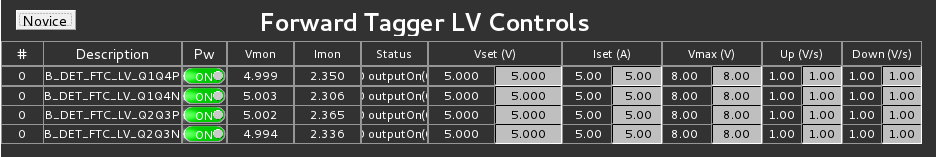
\includegraphics[width=0.9\textwidth]{pics/lvexpert.png}
%    \caption{The LV expert EPICS screen in normal operation.\label{lvexpert}}
%\end{figure}
%%\%\%\%\%\%\%\%\%\%\%\%\%\%\%\%\%\%\%\%\%\%\%\%\%\%\%\%\
%{\em Note, as a safeguard, if one currently tries to use EPICS to set the voltage greater than 5 V or the current greater than 5 A, the request will be ignored by the IOC.}  
%
%\section{High Voltage}
%   \subsection{Changing HV Settings}
%      {\bf NOTE:} Changing voltage settings should be taken care of in coordination with the FT-Cal group (contact M.~Battaglieri). 
% {\bf NOTE:} The FT-Cal HV groups were renumbered for EPICS, and the correspondence map  is available on the following webpage: https://logbooks.jlab.org/entry/3370066.\\
%If for some reason some channels were to drop in gain (or increase) or if the current drawn increases in a group, it might be necessary to change the HV settings in the expert FT-Cal EPICS control (Fig.~\ref{fig:HVControl}). A modification of the voltage will lead to a modification of the gain used by the trigger system, these values need to be updated at the same time!
%  
%\subsubsection{HV Save/Restore}
%A system to save and restore the entire calorimeter's voltage settings is available via the grey button in the HV section of the main Overview page, shown in Figure~\ref{fig:ecal_all}.  If the voltage setpoints are changed, a backup should be made of the new settings.  This must be run as clasrun user in directory  \texttt{/usr/clas12/DATA/burt/FTC\_HV}.
%      An example of the restore window is shown in Figure~\ref{fig:hvrestore}, which is accessible from the FTC Overview screen shown in Figure~\ref{fig:ecal_all}.
%
%%\%\%\%\%\%\%\%\%\%\%\%\%\%\%\%\%\%\%\%\%\%\%\%\%\%\%\%\
%\begin{figure}[htbp]
%\center
%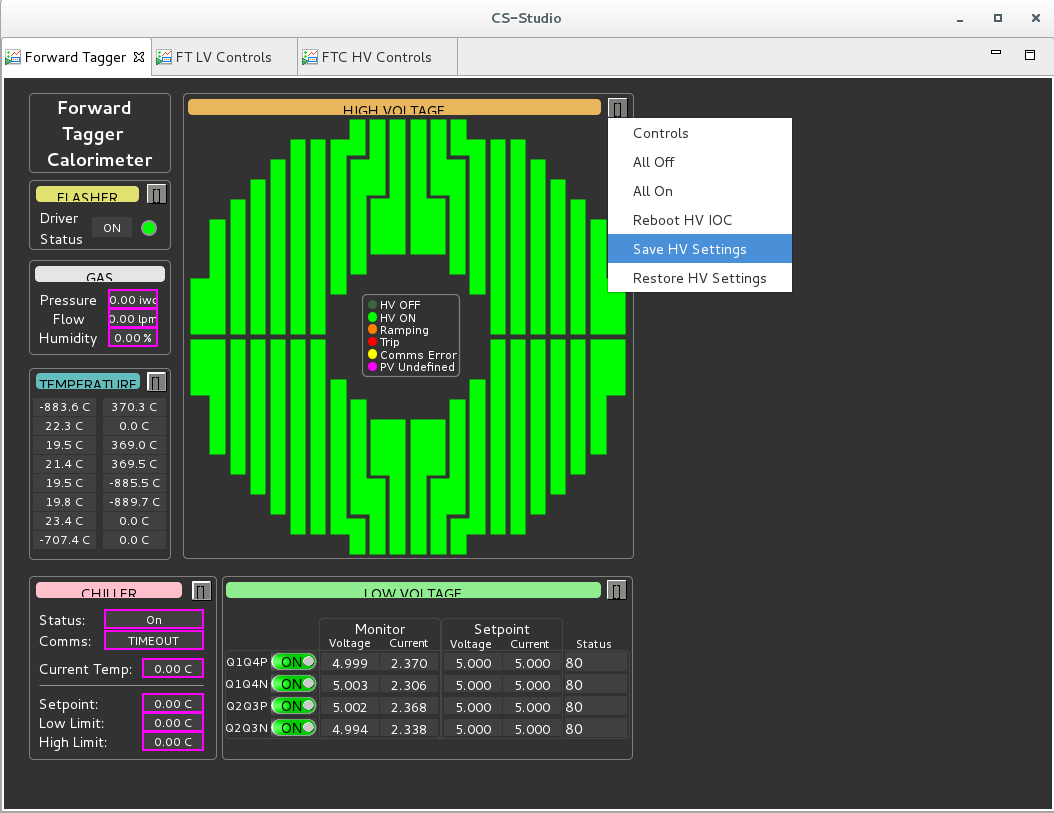
\includegraphics[width=0.85\textwidth]{pics/HVsave_restore.png}
%\caption{\label{fig:hvrestore} Menu button within the High Voltage section of the FTC Overview window which allows the user to save HV setting. To restore simply use the next option below, within the same menu.}
%\end{figure}
%%\%\%\%\%\%\%\%\%\%\%\%\%\%\%\%\%\%\%\%\%\%\%\%\%\%\%\%\
%
%\newpage
%
%\section{LED system for experts}
%%\%\%\%\%\%\%\%\%\%\%\%\%\%\%\%\%\%\%\%\%\%\%\%\%\%\%\%\
%\begin{figure}[htbp]
%\center
%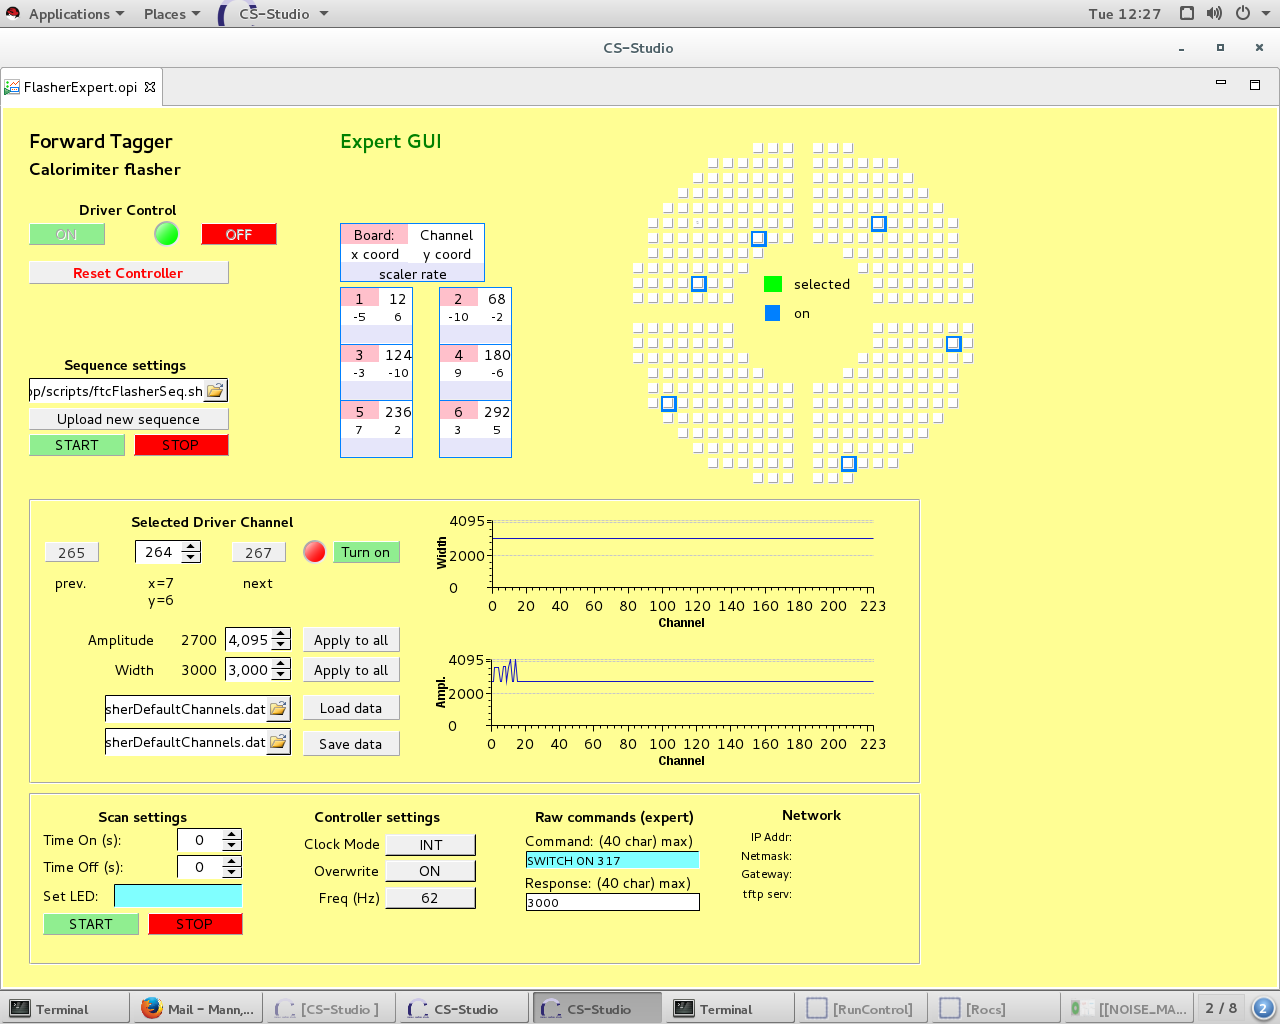
\includegraphics[width=0.85\textwidth]{pics/FTC_flasher_Expert.png}
%\caption{\label{fig:LEDexpert} View of the LED flasher expert controls.}
%\end{figure}
%%\%\%\%\%\%\%\%\%\%\%\%\%\%\%\%\%\%\%\%\%\%\%\%\%\%\%\%\
%
%\begin{enumerate}
%\item{\textbf{Getting There!}}
%\begin{itemize}
%\item Using the Hall-B Epics main window select the option FTC Flasher Expert.\ref{fig:EPICSmain}  Within this GUi the user has master control of all the LED Flasher's capabilities. The User may flash groups or single LED's automatically, set LED amplitudes and widths, send raw commands to the flasher, and control various trigger aspects of the flasher.
%\end{itemize}
%
%\item{\textbf{Novice: Turning on/off}}
%\begin{itemize}
%\item On the Flasher Gui there are two options under driver control ``ON'' and ``OFF''. Before starting anything with the LED system make sure the driver control is on, otherwise all commands you send to the GUi will have no effect. Once finished with your work, remember to switch off the system; if this action is not performed you could unwantingly trigger the system (versus a acalibration run), or flash the APD within the FTCal with an LED while taking an actual run. \ref{fig:LEDexpertTop}
%\end{itemize}
%
%\item{\textbf{Novice: Visual Map}}
%\begin{itemize}
%\item As with the novice window, the user can select single LED's and mouseover each element to determine the component number and LED driver channel. The only limitation of using this map is that, like with the novice version of this Gui, the user will be unable to set Amplitudes, Widths, or turn individual LED's on. \ref{fig:LEDexpertTop}
%\end{itemize}
%
%\item{\textbf{Novice: Sequence}}
%\begin{itemize}
%\item As with the novice window the user can also initiatestart and stop a sequence, with the corresponding buttons on the Gui. This sequece flashes a set of 6 LED's (with exception to the first step, in which only 2 a flashed) at a time for a total of 60 seconds. The 3X2 matrix in the middle shows the current LED's being activated as well as their coordinate positions in the FTCal.  \ref{fig:LEDexpertTop}
%\end{itemize}
%
%%\%\%\%\%\%\%\%\%\%\%\%\%\%\%\%\%\%\%\%\%\%\%\%\%\%\%\%\
%\begin{figure}[htbp]
%\center
%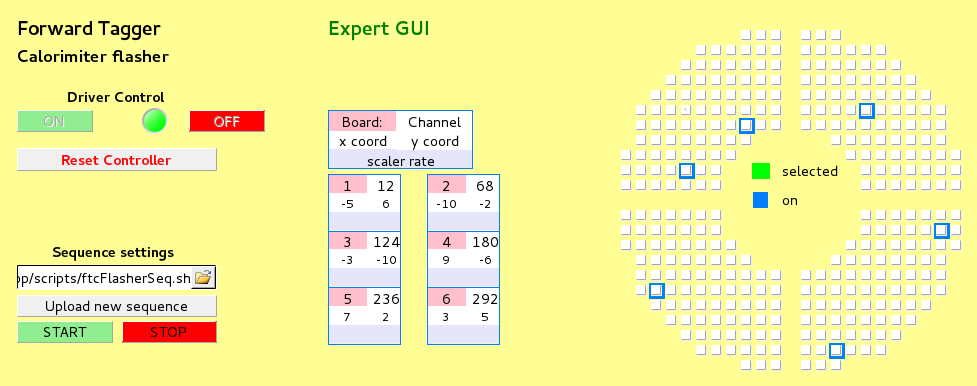
\includegraphics[width=0.85\textwidth]{pics/FTC_flasher_Expert_Top.png}
%\caption{\label{fig:LEDexpertTop} Cropped view of the LED flasher expert controls, showing only the top section.}
%\end{figure}
%%\%\%\%\%\%\%\%\%\%\%\%\%\%\%\%\%\%\%\%\%\%\%\%\%\%\%\%\
%
%\item{\textbf{Expert: Single Selection}}
%\begin{itemize}
%\item In the middle section of the GUi the user will see the options to cycle through each LED in order, starting at (3,11), and transitioning horizontally accross the row when the next LED is selected. Most importantly the user will also be given the opportunity to turn on/off individual LED's for specific channel testing. The numbering system is highlighted in the image below. \ref{fig:LEDnumb} \ref{fig:LEDexpertMid}
%\end{itemize}
%
%\item{\textbf{Expert: Amplitudes and Widths}}
%\begin{itemize}
%\item In the middle section of the Gui, the user will also be allowed to alter the flashing LED's amplitude (brightness), and width (the length of the pulse flash); two graphs on the right side of the window display the distribution of amplitudes and widths for all LEDs. If the user would like to save/load their own settings for all LED's the save/load buttons will perform that task. \ref{fig:LEDexpertMid}
%\end{itemize}
%
%%\%\%\%\%\%\%\%\%\%\%\%\%\%\%\%\%\%\%\%\%\%\%\%\%\%\%\%\
%\begin{figure}[htbp]
%\center
%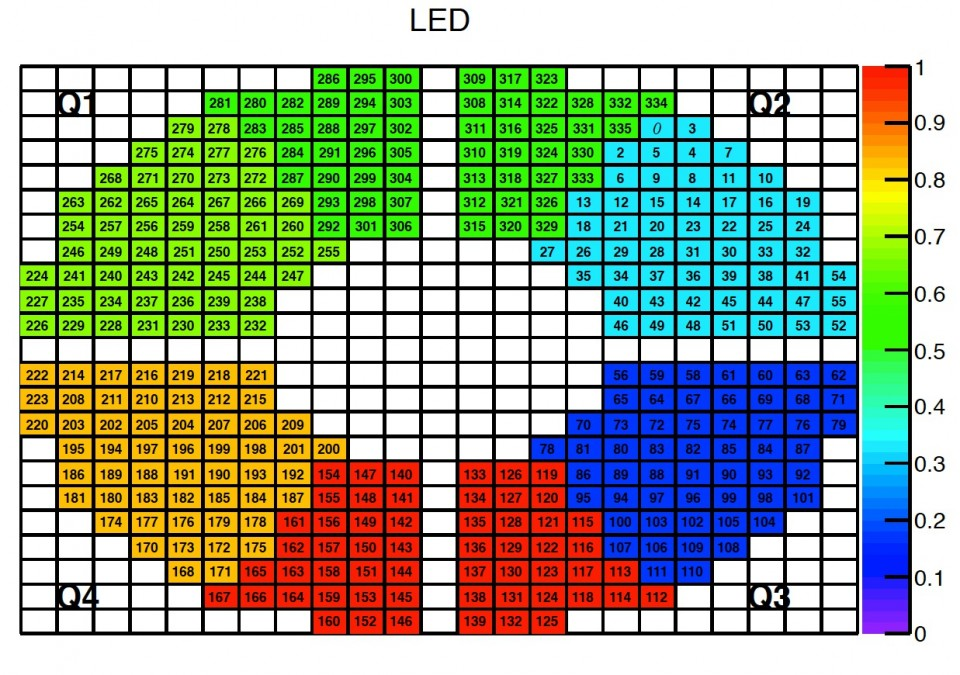
\includegraphics[width=0.85\textwidth]{pics/FT-CalMap-LED_Numb.jpg}
%\caption{\label{fig:LEDnumb} LED number association.}
%\end{figure}
%%\%\%\%\%\%\%\%\%\%\%\%\%\%\%\%\%\%\%\%\%\%\%\%\%\%\%\%\
%
%%\%\%\%\%\%\%\%\%\%\%\%\%\%\%\%\%\%\%\%\%\%\%\%\%\%\%\%\
%\begin{figure}[htbp]
%\center
%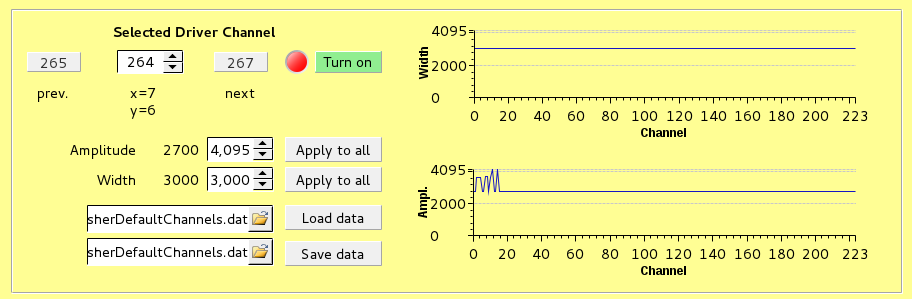
\includegraphics[width=0.85\textwidth]{pics/FTC_flasher_Expert_Mid.png}
%\caption{\label{fig:LEDexpertMid} Cropped view of the LED flasher expert controls, showing only the middle section.}
%\end{figure}
%%\%\%\%\%\%\%\%\%\%\%\%\%\%\%\%\%\%\%\%\%\%\%\%\%\%\%\%\
%
%\item{\textbf{Expert: Controller Setting (Trigger)}}
%\begin{itemize}
%\item Under this column the three buttons displayed allow the user to trigger to the entire system, alter the rates of this trigger, and enable an overwrite function. the  two options related to the trigger are: ``Clock Mode'' and ``Freq (Hz)''.The final button ``Overwrite'' allows the user to continually turn on LEDs without having to turn off the previously selected channel. \ref{fig:LEDexpertBot}
%\end{itemize}
%
%\item{\textbf{Expert: Raw Commands}}
%\begin{itemize}
%\item In order to use this section the user will need to be familiar with the list of raw commands that the flasher can accept. The list of commands is found on the following WIKI page: 
%https://wiki.ge.infn.it/g3wiki/index.php/Monitoring\_system\#For\_dummies in the section title ``List of available commands''  \ref{fig:LEDexpertBot}
%\end{itemize}
%
%
%%\%\%\%\%\%\%\%\%\%\%\%\%\%\%\%\%\%\%\%\%\%\%\%\%\%\%\%\
%\begin{figure}[htbp]
%\center
%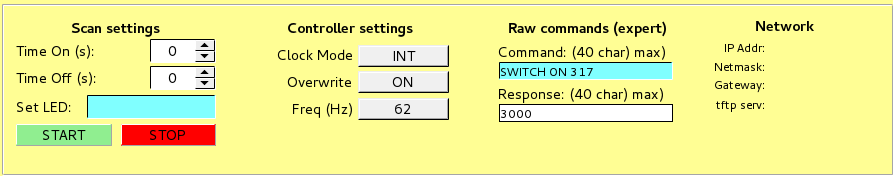
\includegraphics[width=0.85\textwidth]{pics/FTC_flasher_Expert_Bot.png}
%\caption{\label{fig:LEDexpertBot} Cropped view of the LED flasher expert controls, showing only the bottom section.}
%\end{figure}
%%\%\%\%\%\%\%\%\%\%\%\%\%\%\%\%\%\%\%\%\%\%\%\%\%\%\%\%\
%
%\end{enumerate}



\end{document}
